\documentclass[letterpaper]{article}
\usepackage{natbib,alifeconf}
%\usepackage{hyperref}
\usepackage{todonotes}
\usepackage{epstopdf}
\usepackage{soul}

\usepackage[flushleft]{threeparttable}
\usepackage{subcaption}
\usepackage{booktabs}
\setcounter{tocdepth}{3}
\usepackage{array}
\usepackage{float}
\usepackage{dirtytalk}
  \usepackage[font=small]{caption}

\delimitershortfall-1sp
\newcommand\abs[1]{\left|#1\right|}

\title{Evolution of Heterogeneous Cellular Automata in Fluctuating Environments}
\author{First Author$^{1}$, Second Author$^{1,2}$, Third Author$^{1,2}$, Fourth Author$^{1,2}$ \and Fifth Author$^2$ \\
\mbox{}\\
$^1$First affiliation  \\
$^2$Second affiliation \\
corresponding@author.email}

\begin{document}
\maketitle

\begin{abstract}
The importance of environmental fluctuations in the evolution by natural selection of living organisms has been widely noted by biologists and linked to many important characteristics of life such as: modularity, plasticity, genotype size, mutation rate, learning or epigenetic adaptations. In artificial life simulations, however, environmental fluctuations are usually seen as a nuisance rather than an essential characteristic of evolution. HetCA is a heterogeneous cellular automata characterized by its ability to generate open-ended long-term evolution and ``evolutionary progress''. In this paper, we propose to measure the impact of different types of environmental fluctuations in HetCA. Our results indicate that environmental changes induce mechanisms analogous to epigenetic adaptation or multilevel selection. This is particularly prevalent in two of the tested fluctuation schemes, which involve a round-robin inhibition of certain cell types, where a phenotypic selection seems to occur.
\end{abstract}

\section{Introduction}\label{sec:intro}
Environmental changes may include cyclic events such as seasonal changes or a daily cycle of light and darkness, occasional changes such as the introduction of new predator or the potential for a new source of food, or much more radical modifications such as environmental stresses induced by climate change.

Since works such as~\citep{levins1968evolution} or more recently~\citep{jablonka2014evolution}, as well as the attempt to integrate the epigenetic (EIS), developmental (the "Evo-Devo" school \citep{muller2007evodevoextendingtheevolutionarysynthesis}) and environmental (as done by poeple studying "Niche Construction" mechanisms~\citep{laland2016anintroductiontonicheconstructiontheory} dimensions to evolutionary biology, the emphasis has been put on the importance of environmental fluctuations in the evolution by natural selection of living beings. Through these and other works many central mechanisms of evolution have been linked to environmental changes. Modularity, plasticity~\citep{west2005developmental}, size of the genotype, mutation rate and evolvability are some of the most discussed example. 

For \cite{jablonka2014evolution}, changeable environments will unmask variations in the capacity of individuals to make adjustments to changed conditions and therefore promote plasticity. They advance that \say{For a lineage in a constantly changing environment, switching among several alternative heritable states was probably an advantage. While cells in one state survived in one set of conditions, those in other states did better in different circumstances.}\emph{(ibid. p. 318)}. Following that line of thought, constantly changing environment or cycling variations might explain the origin of the Epigenetic Inheritance Systems~\cite{heard2014transgenerationalepigeneticinheritancemythsandmechanisms} as epigenetic mutations are more reversibles and occur more frequently than genetic mutations. To illustrate that, \cite{lachmann1996inheritance} have modelled the effects of cycling variations, such as seasonal or daily cycles, on phenotypical inheritances. Their model predicted that indeed when the investigated cycles are longer than the reproductive cycle but relatively short otherwise, heritable variations produced by non-DNA inheritance systems are likely to be observed. 

In parallel to such studies, a proportion of existing works in artificial life, especially in evolutionary robotics~\citep{floreano2000evolutionary}, considers the issue of environmental variations. Some work in this literature have explicitly define the environment as a driving evolutionary force~\citep{bredeche2012environmentdrivenopenende}. %However and as far as we know, a significant majority of the works in that field still consider environmental changes only as a problem to be solved and nobody has systematically studied the general properties induced by environmental fluctuation over evolutionary dynamics.  %However, it is probably fair to say that, a significant majority of these previous work has either focused on aspects such as normal spatial variation, or has viewed environmental change as a problem to be solved.

Other, such as~\cite{lipson2002origin}, demonstrated a correlation between the modularity and the rate of change of the environment resources, while in \cite{yu2007program} observed that populations exploit neutrality to cope with environmental fluctuations and therefore evolve some sort of evolvability under two alternating objective functions. Both of these two last simulations used Genetic Programming~(GP) and employed explicit fitness functions.

Starting from those observations, we propose an open ended experimental setup that allows to systematically and quantitatively measure the influence of cyclic environmental fluctuations on the course of the evolution of a Cellular Automata (CA). We show that such fluctuations lead to the emergence of processes similar to those exhibited by epigenetic inheritance systems. \todo{Revoir la transition entre ces deux paragraphes: que reprends-t-on des deux études? que change-t-on? quelles sont les hypothese?}

The paper is organized as follow. Section~\ref{sec:hetca} explains the general mechanisms of HetCA simulation and the implementation of environmental fluctuations in HetCA is then detailed in Section~\ref{sec:exsetup}. Section\ref{sec:method} describes the computer experimental setup while we report experimental results in Section~\ref{sec:results}. We discuss the implications of these results in Section~\ref{sec:discuss}. Finally, Section~\ref{sec:conc} concludes the paper.



%\section{Background}\label{sec:bground}
%\input{background.tex}

\section{HetCA}\label{sec:hetca)}
HetCA \citep{medernach2013long} is based on classical two-dimensional CA with several additional features: cells follow a heterogeneous transition function, i.e.~one which depends on their location, inspired by linear genetic programming~(LGP); they can also fall into special \emph{decay} and \emph{quiescent} states; and there is a notion of genetic transfer of transition functions (i.e.~genotypes) between adjacent cells. Decay and quiescent cells do not possess a genotype; all other cells do, and are called \emph{living}; there are 5 different living states; quiescent cells can acquire a genotype from any nearby living cell and therefore become living in turn; decay cells cannot, but become quiescent after a number of consecutive iterations comprised between 375 and 1,875 after decay. Living cells always automatically turn into decay after 7 consecutive iterations spent in any one or several living states (tracked by an ``age'' counter).

We showed that HetCA could exhibit long-term phenotypic dynamics \citep{medernach2013long}, a high level of variance over very long runs, greater behavioral diversity than classical CA, and ``evolutionary progress'' \cite{shanahan2012evolutionary} on three criteria: robustness, size and density of the genotype \citep{medernach2015evolutionary}.
%Moreover, some emergent properties of HetCA are similar to two of the five major eukaryotic innovations which do not appear to have direct prokaryotic predecessors defined in \citep{smith1997major} as : (1)~the eukaryotic chromatin remodelling machinery; (2)~the cell cycle regulation systems; (3)~the nuclear envelope; (4)~the cytoskeleton; and (5)~the apoptosis apparatus \citep{koonin2002origin}. Indeed, in HetCA, the loss of the genotype of the cell as it turns to the quiescent state may seem similar to apoptosis while survival strategies such as the ones depicted in Figure~\ref{foursteps} might akin cell cycle regulation systems \todo{Un peu "Gros" pour la taille des explications non? je veux dire que si c'est vraiment le cas, il faudrait détailler un peu?}

Finally, while there is a lasting debate over the units of selection in evolutionary biology since the origins of the field: genotype selection, phenotype selection, epigenetic selection, behavioral selection, multilevel selection, group selection, and so on \citep{lloyd2012unitsandlevelsofselection,okasha2006evolution}, several of them are potentially included in HetCA. There is genotypic selection of the transition rules, but also phenotypic selection of cell groups able to replicate patterns such as the ones found in the Game of Life. This point is important when one is interested in environmental fluctuations because, as mentioned in the introduction, we anticipate that the existence of frequent environmental fluctuations will promote phenotypic selection over genotypic selection.

\section{Experimental Setup}\label{sec:exsetup}

\subsection{Environmental Fluctuations}
 As in the previous version of HetCA the genotype of an individual is its transition rules encoded with CA-LGP using the function set depicted in Table~\ref{funcSet}. The mutation of genotypes is enabled and we use the Micro/Marco-mutation of CA-LGP as described in \citep{medernach2013long}.

But in order to introduce environmental variations, where the new genotype of a cell was originally randomly chosen among candidate genotypes we vary the likelihood of spread of the genotype of a cell according to the state of this cell. In this new setup, the chances of the candidate genotype of the cell $c$ to be selected are then: \todo{ya pas deux $c$ differents dans cette notation?} $c=K(S_c)/\sum_{i=1}^{n} K(S_{c_i})$ with $S_c$ state of the cell $c$, $K(S)$ likelihood of spread of state $S$ and $n$ number of candidate genotypes. Therefore an environment is characterized by the odds of propagation of the five living states $\{K(S_1),K(S_2),K(S_3),K(S_4),K(S_5)\}$.   
To mimic environmental fluctuations we initialise the simulation with $K(S_i)=1  \forall i \in [1,5]$ and then we regularly change those values from iteration 3000 of the cellular automata. 

We chose to introduce four forms of environmental fluctuations described in Table~\ref{tab:environments}.

\noindent \emph{Short-cycle Fluctuation}: consists of alternating between two environments every 100 iterations of the cellular automaton. We chose to vary the environment every 100 iterations to stay in the same range of frequency as described in Lispson~\citep{lipson2002origin} examples 20 and 100 generations and~\citep{yu2007program} experiments 10, 20 and 50 generations. In fact we consider that a successful reproductive cycle involves passing a cell through the quiescent state. And this should take between two iterations (alternating between the quiescent state and a living state) and seven iterations (if a cell remains in a living state more than seven consecutive iterations it goes to the decay state and can not receive a genotype for an important period).

\noindent \emph{Light Fluctuation}: consists of alternating between five environments every 5000 iterations of the cellular automaton. The first five each prohibit a different state from the five living state, the latter gives equal chance to each of the five states.

\noindent \emph{Strong Fluctuation}: consists of alternating between twelve environments every 5000 iterations of the cellular automaton. The first eleven each prohibit a different combination of two states from the five living states, the latter gives equal chance to each of the five states.

\noindent \emph{Gradual Fluctuation}: is similar to strong fluctuation except that it includes a transition phase of $T=60$ iterations in between two environments where likelihood of spread of state values progressively switch from the value a previous environment to the ones of the new environment. Over this phase the state spreading is defined by the following formula : $K(S,t)=K_p(S) \times (T-t) + K_{p+1}(S) \times t$ where $t$ is the number of iterations completed since the beginning of the transition phase; $K_p(S)$ and $K_{p+1}(S)$ are likelihood of state spread $S$ for the current environment and the next environment respectively.

\emph{Short-cycle fluctuation} may be analogous to the circadian rhythms for some bacteria: very regular cycles in which these organisms have enough time to reproduce several times. While \emph{light fluctuation} may be similar to seasonal fluctuations and \emph{strong and gradual fluctuations} would akin ecological crisis. Although, owing to the variety of both biological temporal rhythms and reproductive cycles, the relevance of these analogies may be limited. 

%\subsection{Common Settings}\label{sec:commonset}

\begin{table}
\scriptsize
\centering
  \begin{tabular}{l>{\centering}p{0.6\columnwidth}}
  \toprule%
    \textbf{op. name}	& \textbf{action} on inputs $(x,y)$\tabularnewline
 \toprule%   
    abs			& $|x|$ \tabularnewline
    plus		& $x+y$ \tabularnewline
    delta		& 1, if $|x-y| < 1/10000$; 0 o.w. \tabularnewline
    dist		& $|x-y|$ \tabularnewline
    inv			& $1-x$ \tabularnewline
    inv2		& safeDiv($1, x$) \tabularnewline
    magPlus		& $|x+y|$ \tabularnewline
    max			& $\max \{x,y\}$ \tabularnewline
    min			& $\min \{x,y\}$ \tabularnewline
    safeDiv		& $x/y$ if $|y| >  1/10000$; 1 o.w. \tabularnewline
    safePow		& $x^y$, if defined; 1 o.w. \tabularnewline
    thresh		& 1, if $x > y$; 0 o.w.\tabularnewline
    times		& $xy$ \tabularnewline
    zero		& 1, if $|x| < 1/10000$; 0 o.w. \tabularnewline
\bottomrule%
  \end{tabular}
    \caption{\textbf{Function set}. \label{funcSet}}
\end{table}


\section{Simulations}\label{sec:method}

For each form of environmental fluctuation and the stable non fluctuating environment we performed 50 simulations which make a total of $4\times50=200$ runs. Each run last 500000 iterations with the parameters listed in Table~\ref{settings}. In following section we report average value with standard deviations.

\begin{table}
\scriptsize
\centering
\begin{tabular}{l>{\centering}p{0.2\columnwidth}}\toprule%
Parameter & Value \tabularnewline
\toprule%
Number of living states & 5\tabularnewline
Successive living iterations before decay & 7\tabularnewline
Number of iterations for decay & 375-1875\tabularnewline
Direct transition to decay & enabled\tabularnewline
Size of the grid & 500x500\tabularnewline
Grid boundaries & toric grid\tabularnewline
Transition Rule~(TR) & CA-LGP\tabularnewline
Maximum (TR) size & 50 program statements\tabularnewline
Genotype copy neighbouring  & Von Neumann \tabularnewline
Transition rule neighbouring & Moore\tabularnewline
\bottomrule%
\end{tabular}
\caption{ \textbf{HetCA parameters}.}
  \label{settings}
\end{table}

\subsection{Genotype Size}
We use the number of program statements ($n_{prog}$) as a measure of the genotype size and compute the average size of all the current genotypes of a run every 2500 iterations. We then report the average and standard error among all the fifty runs sharing the same settings.

\subsection{Changes induced by environmental fluctuation}
If, as postulated in \citep{jablonka2014evolution}, the introduction of environmental changes leads to the selection of plasticity or to the emergence of phenotypic selections\footnote{Similar to the epigenetic inheritance system} using easily reversible phenotypic mutations, then phenotypes from different individuals of the same lineage observed while environmental conditions are similar should be relatively close even though individuals from their lineage evolved in other environmental conditions between these measures. While, if the adaptation to each environmental change is done exclusively through the selection of classical irreversible genotypic mutations, these phenotypes shall be quite different, despite the potential evolutionary convergence. That is why we want to develop a metric to measure phenotypic proximity between two iterations of the CA. To do this we simply compare the proportions of living cells in different states among the possible states. The phenotypic difference $\sigma(t_1,t_2)$ between two iterations $t_1$ and $t_2$ is then calculated as:
$$\sigma(t_1,t_2) = \sum_{s=1}^5 \abs{ \frac{N(s,t_1)}{N(t_1)}-\frac{N(s,t_2)}{N(t_2)}}$$ where $N(s,t)$ is the number of cells at the state $s$ for iteration $t$ and $N(t)=\sum_{s=1}^5 N(s,t)$ is the total number of living cells.

Every 5000 iterations $t$ of the CA we perform two phenotypic comparison with an iteration $t'$ such as $t'\in[t-55000;t-60000]$. The first phenotypic comparison aims to compare two similar environment and therefore we choose $t'$ such as $E(t')=E(t)$. The second phenotypic comparison aims to compare two disimilar environment and therefore we choose $t'$ such as $E(t')=E(t+f)$.  

\subsection{Diversity}
We use the true diversity index of order two to measure phenotypic and genotypic diversity at every iteration $t$ of the CA. Phenotypic diversity is therefore: $$^2D_p(t)=\left(\sum_{s=1}^5 \left(\frac{N(s,t)}{N(t)}\right)^2\right)^{-1}$$ while genotypic diversity is: $$^2D_g(t)=\left(\sum_{g=1}^{K(t)} \left(\frac{N(g,t)}{N(t)}\right)^2\right)^{-1}$$ with $K(t)$ number of distinct genotypes for iteration $t$ and $N(g,t)$ number of cells sharing the genotype $g$ at iteration $t$, note that $N(t)=\sum_{s=1}^5 N(s,t)=\sum_{g=1}^{K(t)} N(g,t)$.

\subsection{Homogenous Test}
We also collect the \emph{most common genotype}~(most frequently occurring) in iterations 2500\footnote{\citep{medernach2015evolutionary}  has shown that the most common genotypes during the first iterations of HetCA were unlikely to have a viable survival strategy, therefore we chose to collect genotypes from iteration 2500}, 102500, 202500, 302500, 402500 and 500000. We tested all genotypes collected in homogeneous simulations, i.e. without mutation and where all cells are initialized with the tested genotype. We then tested each collected genotype in every four environment used, thus performing $4\times50\times6\times4=4800$ runs. We set the maximum duration of these runs to 60000 iterations so that runs performed with \emph{Strong Fluctuations} last long enough to go through all environments. Sometimes the genotype is not adapted to the environment and living cells extinct\footnote{By all turning to decay or quiescent state.} before the end of the 60000 iterations. We consider an Homogenous test to be successful if living cells doesn't extinct before 60000 iterations. We report the success rate of those simulations and the ending iterations of the runs that fail o reach iteration 60000. 

\subsection{Regular phenotype characterization and Phenotype disturbance} 
In HetCA, to survive in the long term the genotypes must regularly release cells by transforming them into quiescent cells without genotypes. This generates patterns and cycles which are quite easy to observe in homogeneous simulations where a single genotype is tested as shown in Figure~\ref{foursteps}~(a), but also observable, although with more difficulty, in normal, heterogeneous, HetCA simulations as seen in Figure~\ref{foursteps}~(b).That is why, to characterize phenotypes, we found it useful to measure these cycles as well as out-of regularities. At every iteration $t>8$ of the homogenous genotype test, we compare the states $S_t$ and $S_{t-1}$ of each cell to their anterior state during the eight previous iterations of the CA. We then measure whether this sequence of two states is repeated during these eight previous iterations, and if so what is its periodicity $p$ such as $p=\min p \in [2;7], S_t=S_{t-p} \wedge S_{t-1}=S_{t-1-p}$. We use here a sequence of two states because, if the genotype of a cell adopts a stable strategy, i.e. repeats a sequence of states, this sequence must contain a minimum of two states in order to ensure the survival of the genotype -- the quiescent state and one of the living states. We have chosen to limit ourselves to a comparison of the eight previous iterations to reduce the computational cost and because the limit of the seven consecutive live iterations before decay involves, for a successful regular phenotype, a maximum periodicity of seven iterations for the quiescent state. We perform this measure only if there is at least a living state among the last two states and no state decay. We then report, for each iteration $t$ of the CA, the phenotype disturbance $$P(t) = \sum_{p=1}^7 \abs{ \frac{N(p,t)}{N(t)}-\frac{N(p,t-1)}{N(t-1)}}$$ with $N(p,t)$ total number of cell with $p$ periodicity for iteration $t$. This measure is quite rough but it is interesting because here, unlike phenotypic difference, it is not directly based on the states of the cells and therefore seems less available able to be directly correlated to state's likelihood of spread.
 
\begin{figure}[h]
\centering
\begin{tabular}{cc}
    \includegraphics[width=0.45\columnwidth]{img/4steptransition}& \includegraphics[width=0.45\columnwidth]{img/cyclesReal}\\
    (a) & (b)
\end{tabular}
\caption{\textbf{Six steps survival strategy}: (a) from a genotype extracted from a HetCA simulation in a stable environment and in a randomly initialized homogenous CA and (b) from a HetCA simulation with \emph{Short-cycle Fluctuations}. }
  \label{foursteps}
\end{figure}
 
%\begin{figure}[h]
%\centering
%\caption{\textbf{Six steps survival strategy} }
%  \label{fourstepsreal}
%\end{figure}








\section{Results}\label{sec:results}
\subsection{Genotype Size \& Genotype mutations}

Figure~\ref{fig:Size} shows genotype size under the various study conditions. The size is bounded (50 is the maximum size) and it limits the differences between those environments as most simulations converge towards this limit, however, one can clearly see here that \emph{Short-cycle Fluctuation} restrict the size of the genotypes while other forms of fluctuations do not appear to have any effect on genotype size. This size reduction could be a way to increase the impact of genotypic mutations on the phenotype. Indeed even if in LGP, when a mutation occurs, its effect is proportional to the size of the genotype, long genotype may enable redundancy information to stabilize the phenotype. Figure~\ref{fig:Size} depicts the amount of accumulated mutation of the most common individual. The amount of mutations separating the current most common individual from individuals created at initialization of the simulation. It is not surprising that more mutations are selected when there are environmental fluctuations\footnote{And those seem to depend more on the strength of these fluctuations than on their periodicity.} but we note that the proximity of strong fluctuation and Short Cycle fluctuations indicates that their genotype difference in size is not only explained by differences in the number of selected mutations.


\begin{figure}[h]
\centering
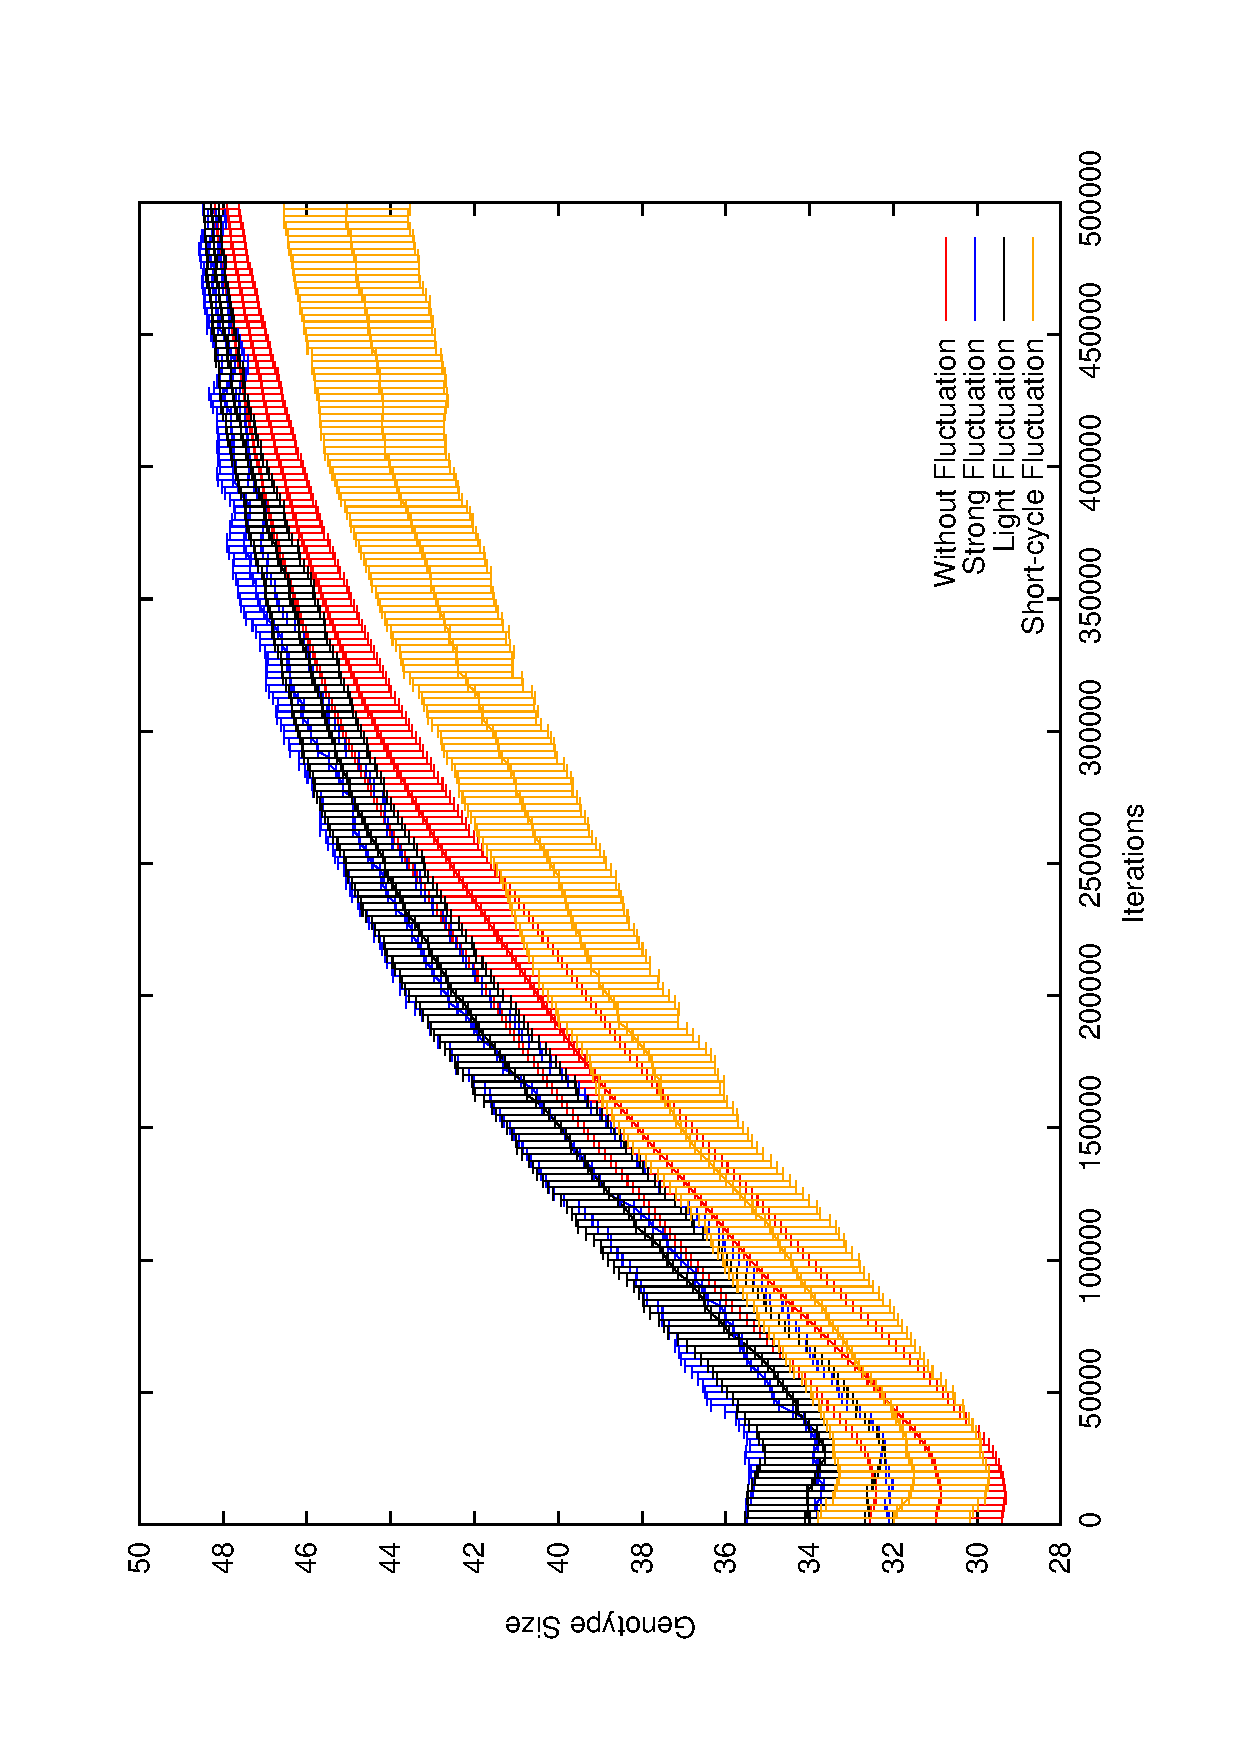
\includegraphics[width=0.7\columnwidth, angle =-90 ]{img/Size}
\caption{\textbf{Size of genotypes}. 
}
\label{fig:Size}
\end{figure}

\begin{figure}[h]
\centering
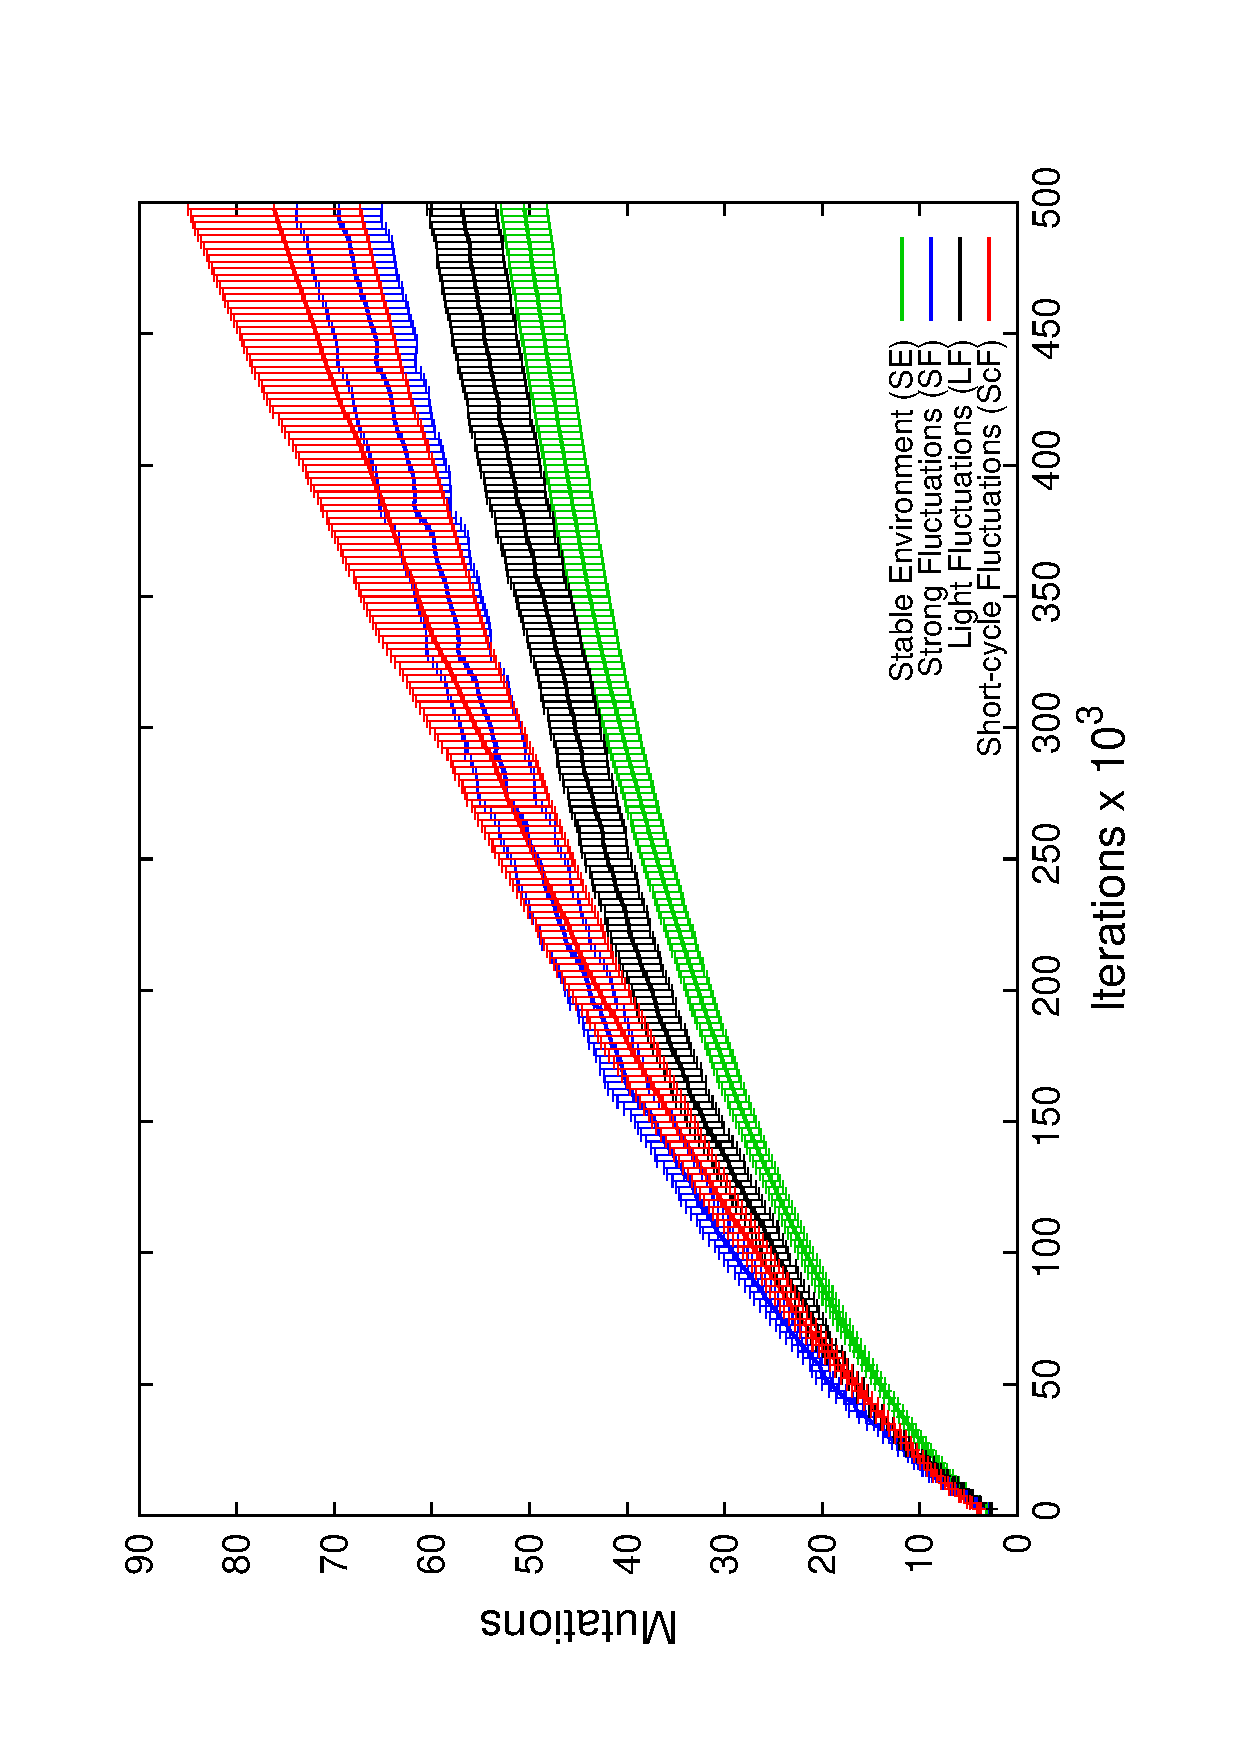
\includegraphics[width=0.7\columnwidth, angle =-90 ]{img/Mutations}
\caption{\textbf{Mutations of genotypes}.
}
\label{fig:Mutations}
\end{figure}

\subsection{Phenotypic Comparison}
Figure~\ref{fig:disimilar} depict phenotypic comparison of disimilar environment, one can see that the impact of environmental fluctuations decreases quickly for \emph{Short-cycle  Fluctuation} while it remains very high for other forms of environmental fluctuations. We also noted that the phenotypic difference of \emph{Short-cycle fluctuations} remains most of the time under the phenotypic differences of the \emph{stable environment}. This suggests a selection of a single phenotype, robust in both environments. Figure~\ref{fig:similar} depict phenotypic comparison of similar environment, it can be observed that, for \emph{Light and Strong fluctuations}, phenotypic differences are much lower than in Figure~\ref{fig:disimilar}, in particular, for \emph{Light fluctuations} they are, most of the time, not significantly different from \emph{stable environment}. The fact that the phenotypic changes induced by environmental fluctuations can be undone by a return to the original environment suggests either plasticity or a strong evolutionary convergence.

\begin{figure}[h]
\centering
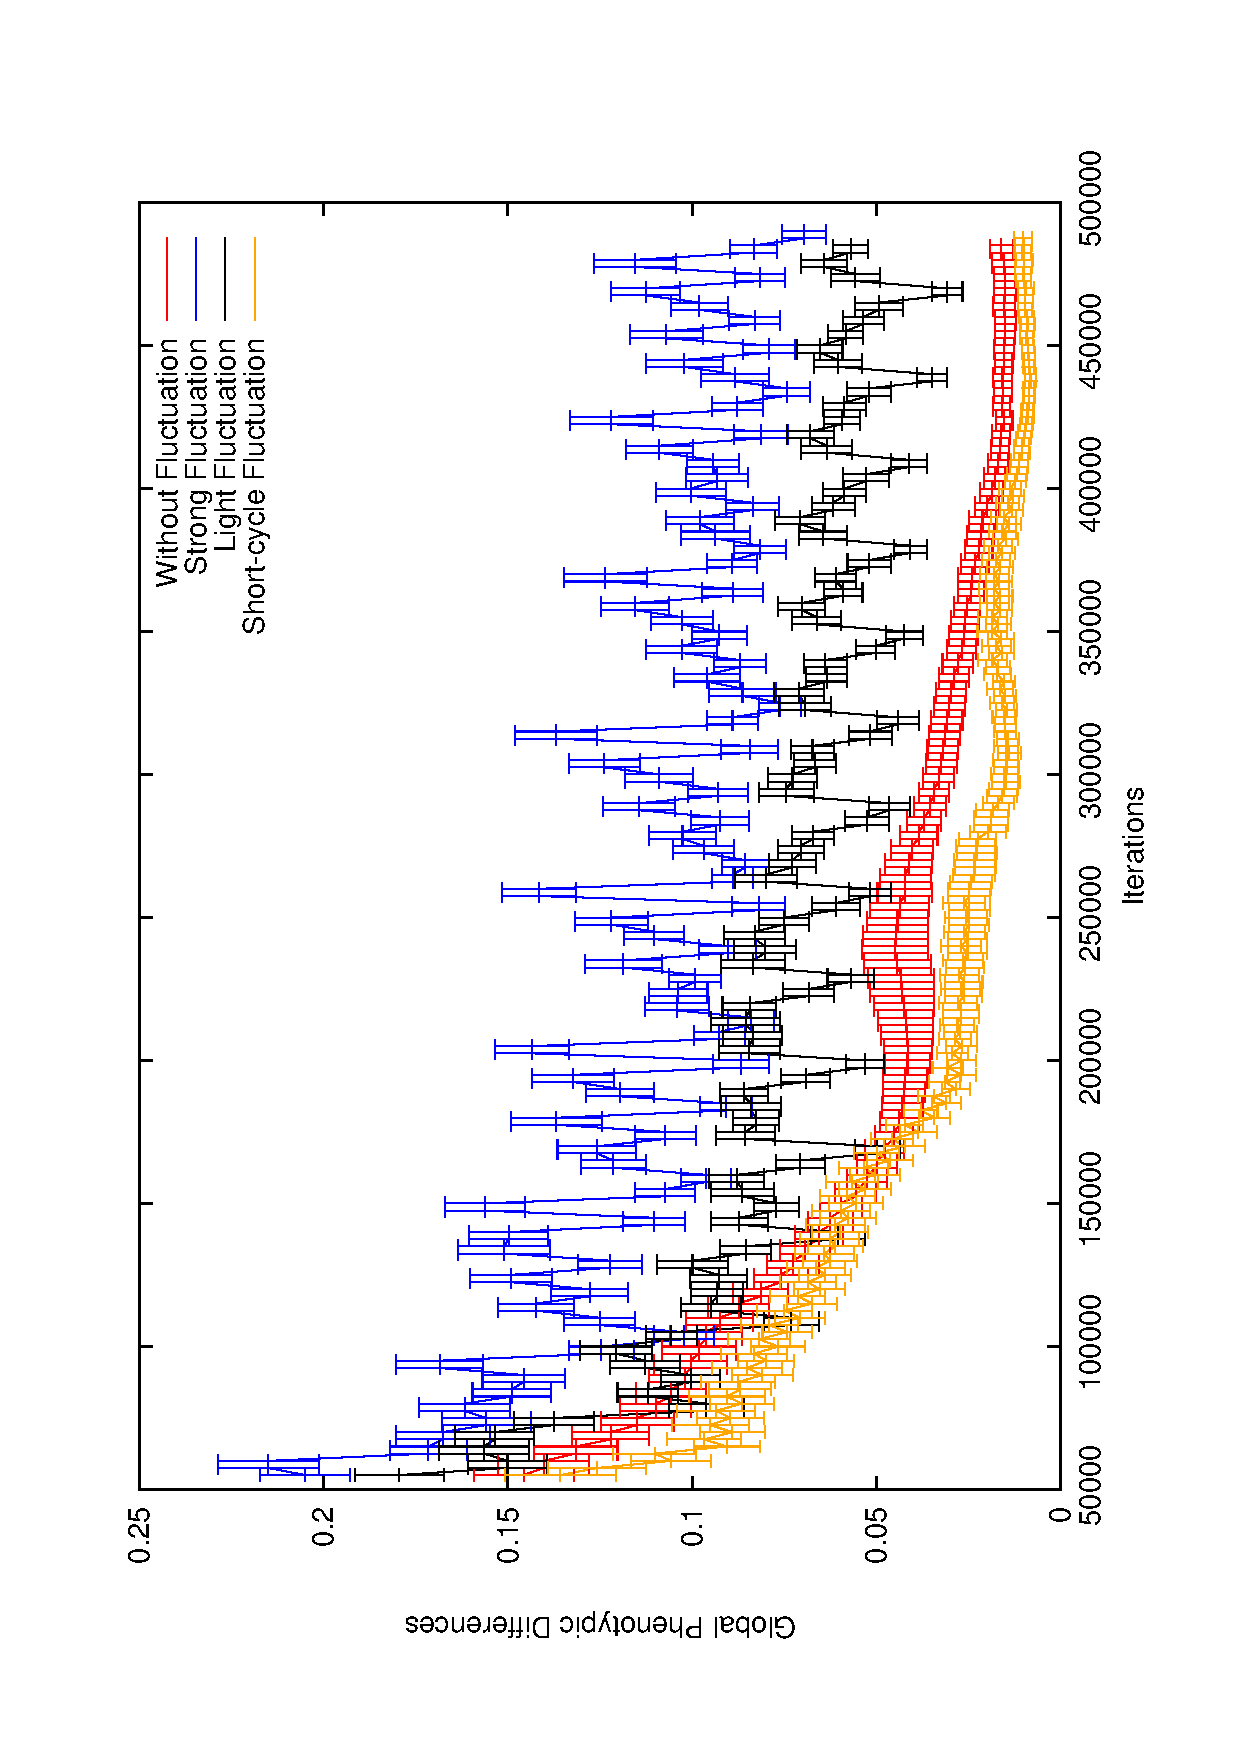
\includegraphics[width=0.7\columnwidth, angle =-90 ]{img/diffProp}
\caption{\textbf{phenotypic comparison of disimilar environments}.}
\label{fig:disimilar}
\end{figure}

\begin{figure}[h]
\centering
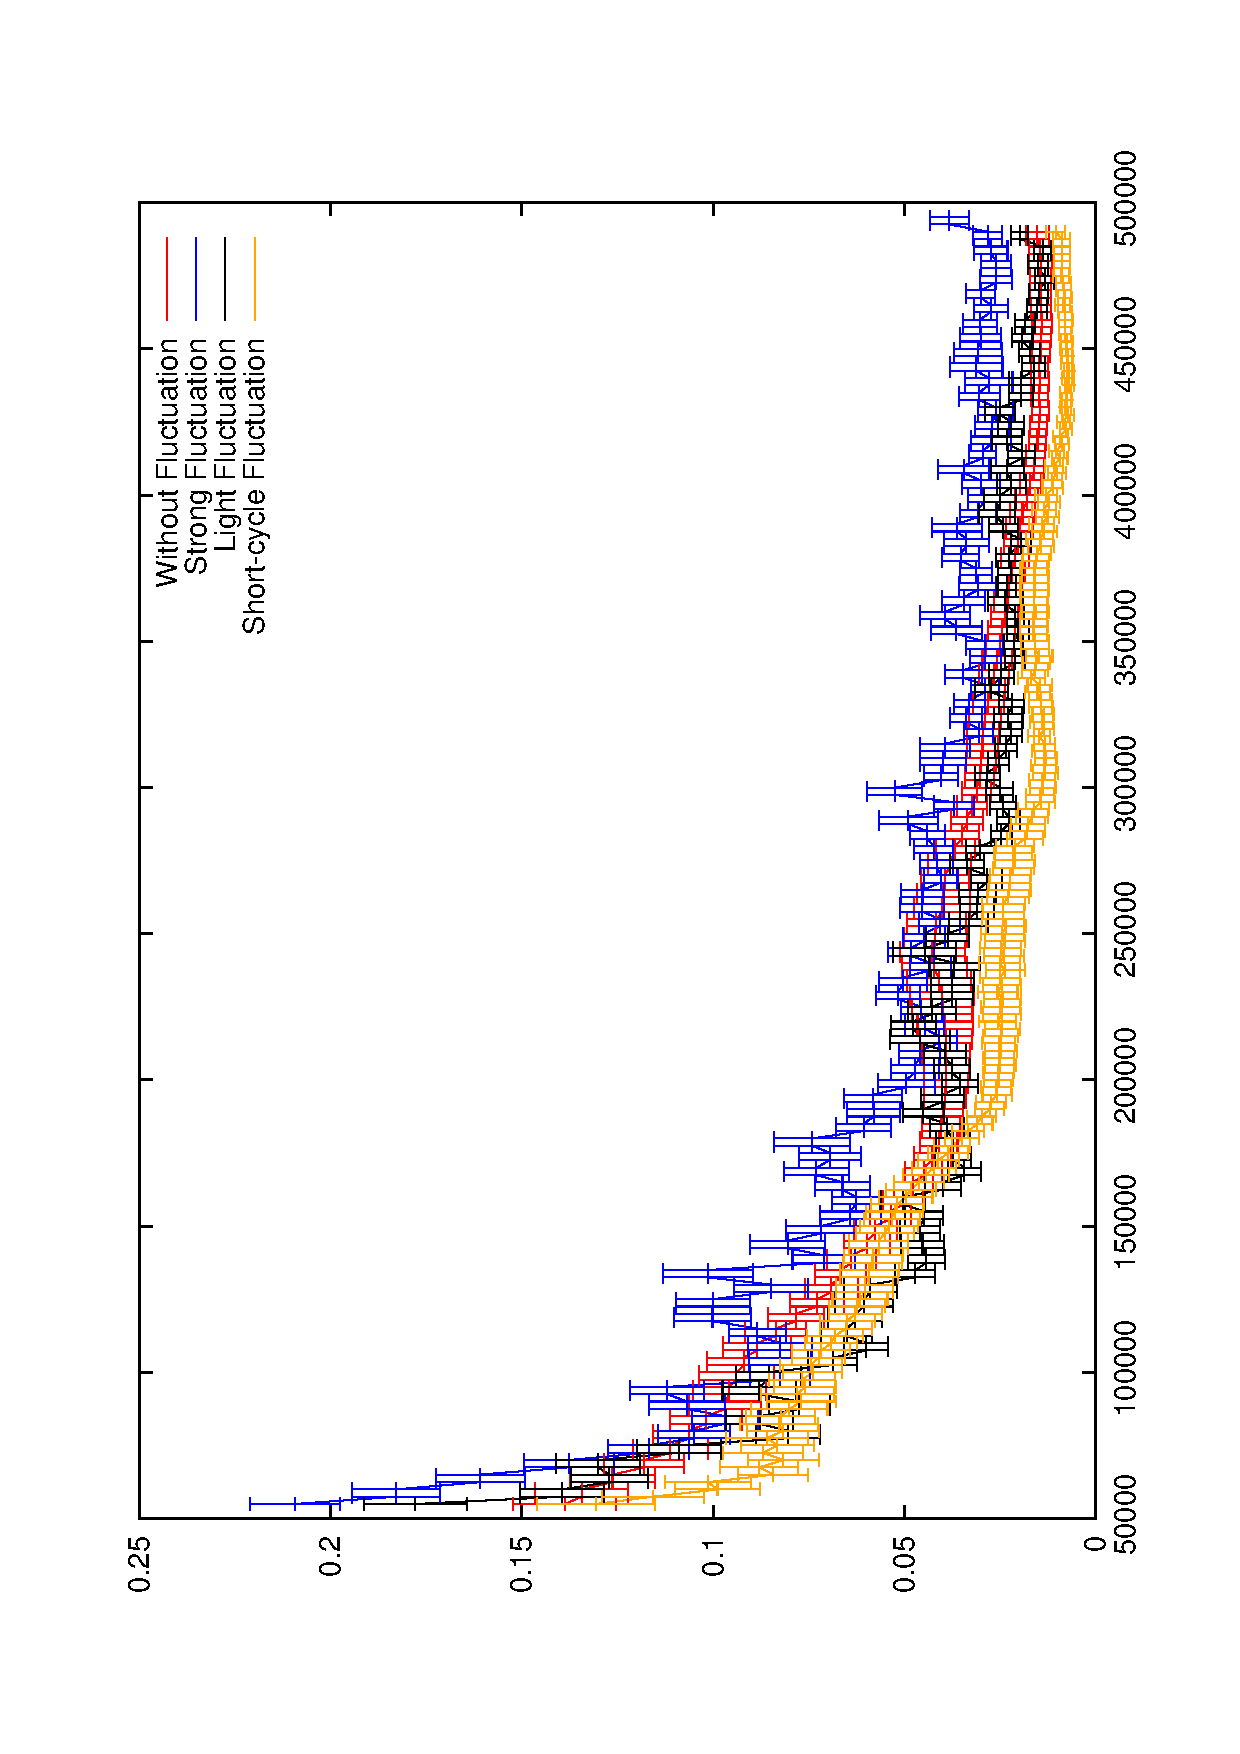
\includegraphics[width=0.7\columnwidth, angle =-90 ]{img/ProgressProp}
\caption{\textbf{phenotypic comparison of similar environments}.}
\label{fig:similar}
\end{figure}




\subsection{Phenotypic and Genotypic Diversity}
Figure \ref{fig:phenodiv} and \ref{fig:genodiv} depict the average phenotypic and genotypic diversities. The low phenotypic diversity of \emph{Short-cycle fluctuations}, suggests the existence in this configuration of a dominant phenotype rather stable over time. While the relatively high phenotypic diversity of \emph{Light and Strong fluctuations} combine with a relatively low genotypic diversity might suggest the existence strong phenotypic selection and therefore some form of plasticity.



\begin{figure}[h]
\centering
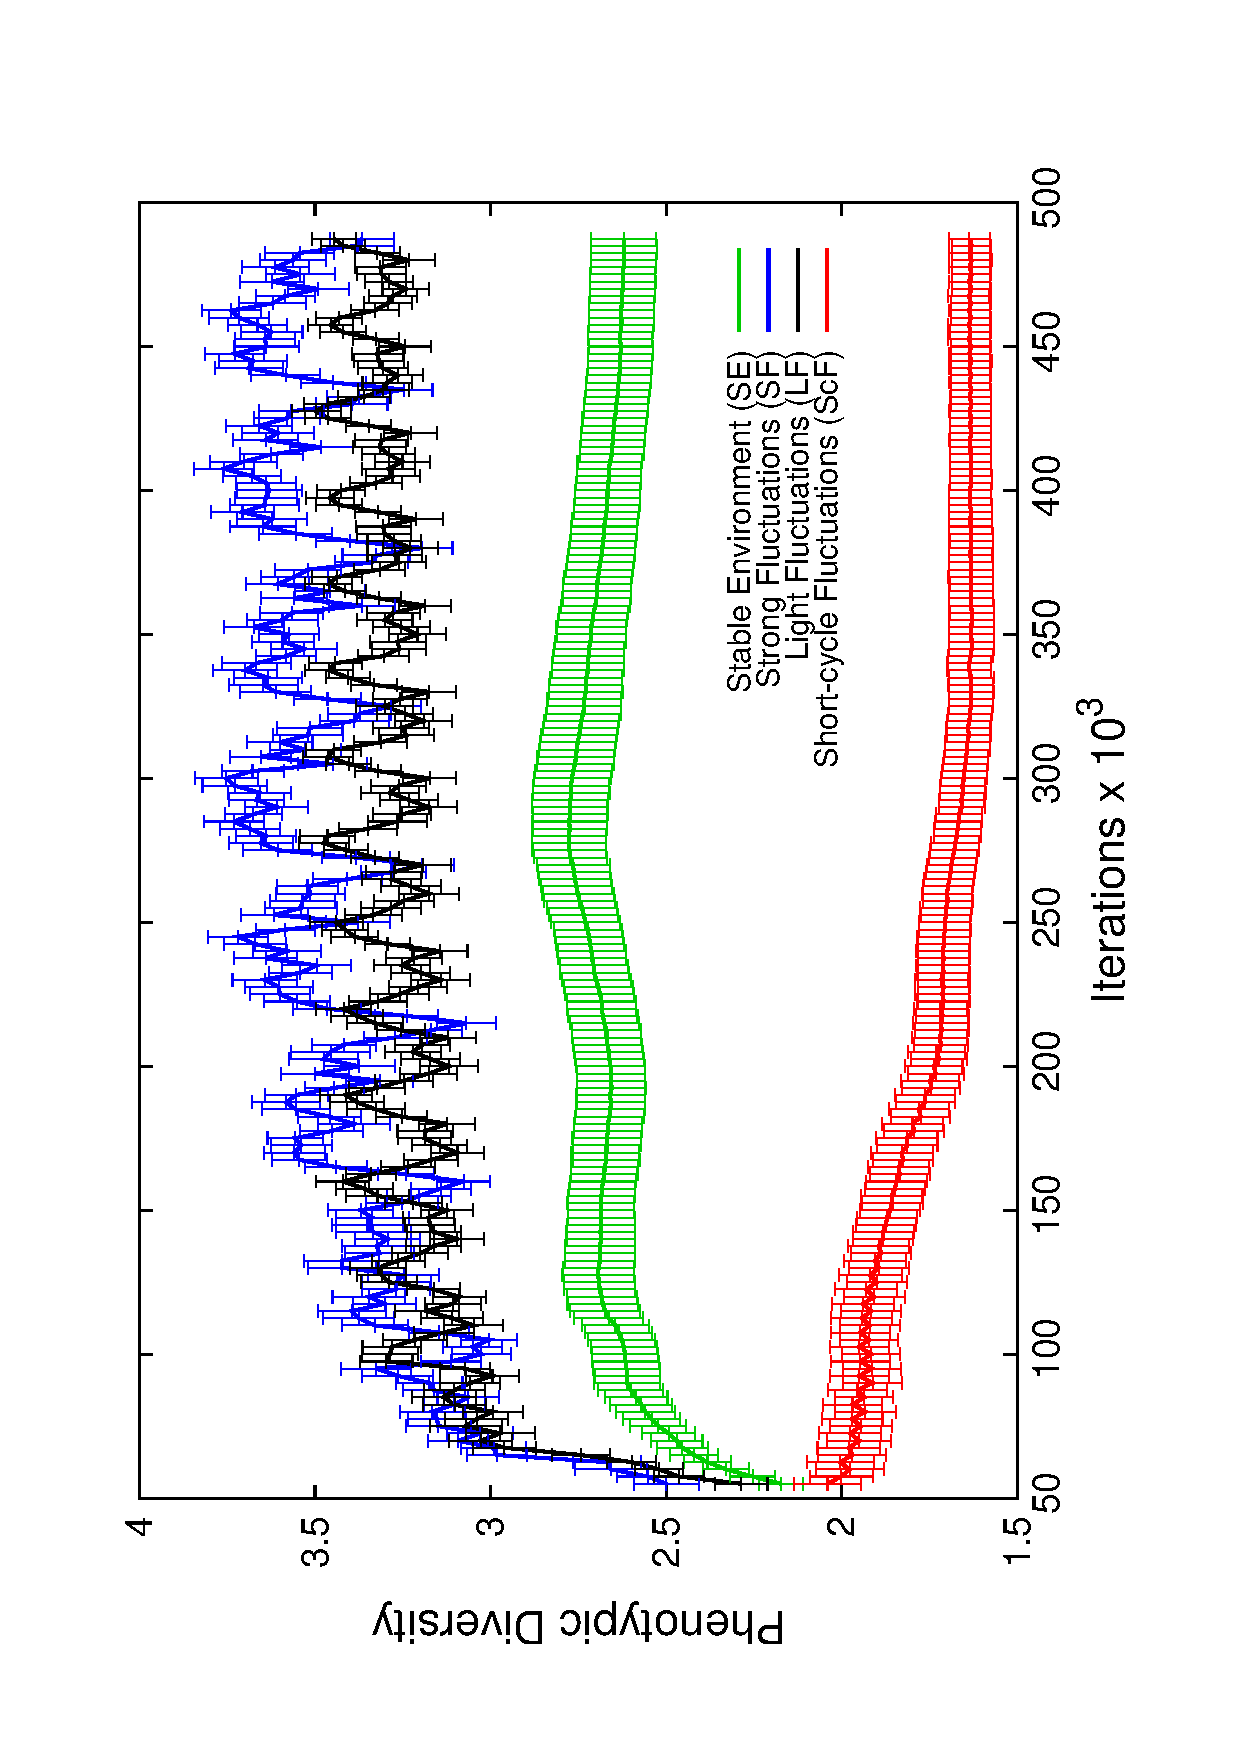
\includegraphics[width=0.7\columnwidth, angle =-90 ]{img/PhenoDiv}
\caption{\textbf{Phenotypic diversity}.}
\label{fig:phenodiv}
\end{figure}

\begin{figure}[h]
\centering
\includegraphics[width=0.7\columnwidth, angle =-90 ]{img/GenoDiversity}
\caption{\textbf{Genotypic diversity}.}
\label{fig:genodiv}
\end{figure}

\subsection{Success Rate and ending iteration of homogenous test}
Success rates of genotypes in different homogenous simulations are reported in Figure \ref{fig:survrate} using normal approximation interval with a confidence of 95\%. Looking at the different success rates we can first order the different tested environment by increasing difficulty : \emph{Stable Environment}; \emph{Short-cycle Fluctuations}; \emph{Light Fluctuations} ; \emph{Strong Fluctuations}. The fact that the \emph{stable environment} offers the lowest challenge is not surprising. Similarly the fact that \emph{Light Fluctuations} are less difficult than \emph{Strong fluctuations} is quite expected. We believe that the slightest difficulty in \emph{Short-cycle Fluctuations} than in \emph{Light Fluctuations} is due to the reduced number of different environment in \emph{Short-cycle Fluctuations} and, in particular, to the fact that, in this configuration, one of the living state is allowed for all environments $K(S_3)=1$. It is also noteworthy that individuals from \emph{Strong and Light Fluctuations} seem relatively robust in various environmental configurations while those from \emph{Short-cycle Fluctuations} doesn't seem robust outside environmental conditions in which they evolved. Moreover, among genotypes collected from iteration 102500, these same individuals are the only ones that do not reach a 100\% survival ratio in a stable environment.


\begin{figure*}[h]
\centering
\includegraphics[width=2\columnwidth]{img/testSurvivingRates}
\caption{\textbf{Success Rate of genotypes in Homogenous Tests}.}
\label{fig:survrate}
\end{figure*}

\subsection{Ending iteration}

Figure \ref{fig:ending} depict the last iteration with living cells of homogenous runs that didn't reach 60000. Note that \emph{Short-cycle Fluctuation} genotypes failures are concentrated around iteration 15000 on \emph{Light Fluctuation} homogenous test and around iteration 25000 on \emph{Strong Fluctuation} homogenous test. This corresponds, for these two configurations, to the first environment for which $K(S_3)=0$, while $K(S_3)=1$ for every environment used in \emph{Short-cycle Fluctuation}. But we also see that some of the genotypes from \emph{Short-cycle Fluctuation} fail during the early iterations of Homogenous test regardless of the used configurations including \emph{Stable Environment} and \emph{Short-cycle Fluctuation}.

This imply that the ecosystem resulting the evolutionary history of individuals plays an key role in their ability to survive. This failure reminds the impossibility of saving species by the unique preservation of their DNA mentioned in \cite{jablonka2014evolution}: \say{You would have to reconstruct the community, and often these communities are very old, with historical memories that are stored in their epigenetic and behavioral systems. These are part of their “identity,” part of their stability. You cannot freeze these memories: they have to be maintained and transmitted through use, so you cannot reconstruct the communities from their component parts.}\emph{(ibid. p. 363)}.

\begin{figure}[H]
\begin{subfigure}{.25\textwidth}
  \centering
  \includegraphics[width=.7\linewidth, angle =-90]{img/boxendingsFailedstable.eps}
  \caption{Stable environment.}
  \label{fig:sfig1}
\end{subfigure}%
\begin{subfigure}{.25\textwidth}
  \centering
  \includegraphics[width=.7\linewidth, angle =-90]{img/boxendingsFailedvariation.eps}
  \caption{Strong Fluctuation.}
  \label{fig:sfig2}
\end{subfigure}

\begin{subfigure}{.25\textwidth}
  \centering
  \includegraphics[width=.7\linewidth, angle =-90]{img/boxendingsFailedvariationLight.eps}
  \caption{Light Fluctuation.}
  \label{fig:sfig2}
\end{subfigure}%
\begin{subfigure}{.25\textwidth}
  \centering
  \includegraphics[width=.7\linewidth, angle =-90]{img/boxendingsFailedvariationSmall.eps}
  \caption{Small Fluctuation.}
  \label{fig:sfig1}
\end{subfigure}
\caption{Last iteration with living cells of homogenous runs that didn't reach 60000. iterations.}
\label{fig:ending}
\end{figure}



\subsection{Phenotypic Densities}
Figure \ref{fig:density} depict the density of phenotypes as measured in homogeneous tests. 

\begin{figure}[H]
\begin{subfigure}{.25\textwidth}
  \centering
  \includegraphics[width=.7\linewidth, angle =-90]{img/boxdensitystable.eps}
  \caption{Stable environment.}
  \label{fig:sfig1}
\end{subfigure}%
\begin{subfigure}{.25\textwidth}
  \centering
  \includegraphics[width=.7\linewidth, angle =-90]{img/boxdensityvariation.eps}
  \caption{Strong Fluctuation.}
  \label{fig:sfig2}
\end{subfigure}

\begin{subfigure}{.25\textwidth}
  \centering
  \includegraphics[width=.7\linewidth, angle =-90]{img/boxdensityvariationLight.eps}
  \caption{Light Fluctuation.}
  \label{fig:sfig2}
\end{subfigure}%
\begin{subfigure}{.25\textwidth}
  \centering
  \includegraphics[width=.7\linewidth, angle =-90]{img/boxdensityvariationSmall.eps}
  \caption{Small Fluctuation.}
  \label{fig:sfig1}
\end{subfigure}
\caption{Density of Genotype : Each genotype density is processed in four possible different environments.}
\label{fig:density}
\end{figure}




\section{Analysis}
\subsection{Environmental Transitions} 
Figure \ref{fig:trans} depicts the average transition between environments in different homogenous runs. To compute this typical transition we averaged phenotype disturbance calculated at iterations $[t-40; t + 40] \forall t \in T_r	
\ge 5000$ where $T_r$ is the set of every iteration of the run $r$ such that a transitions between environments occurs, i.e. $E(t) \ne E(t+1)$. Figure  \ref{fig:transonly} shows the different average transitions of ScF genotypes tested a homogeneous test with the same fluctuations. We can see that phenotypes of the genotypes collected later in the evolutionary process are less sensitive to environmental fluctuations. Conversely, as reported of Figure \ref{fig:transli}, the phenotypes of genotypes from SF keep the same high sensitivity regardless of the iteration in which they were collected. Finally the figures \ref{fig:transst} and \ref{fig:transstest} compare the average transitions in homogeneous test with ScF and SF of genotypes collected at iteration 500000 in the four different configurations. Again, it can be seen there that the phenotype of ScF is much more stable than others in its original environment. On the contrary, tested in SF this genotype is very sensitive to transitions. High sensitivity to fluctuations includes both individuals which developed plasticity and those which fail to resist the environement fluctuations.


\begin{figure}[H]
\begin{subfigure}{.25\textwidth}
  \centering
  \includegraphics[width=.7\linewidth, angle =-90]{img/Sucavg499999variationb.eps}
  \caption{SF on genotypes from i:50000.}
  \label{fig:transst}
\end{subfigure}%
\begin{subfigure}{.25\textwidth}
  \centering
  \includegraphics[width=.7\linewidth, angle =-90]{img/SucavgvarValidvariationb.eps}
  \caption{SF on genotypes from SF.}
  \label{fig:transli}
\end{subfigure}

\begin{subfigure}{.25\textwidth}
  \centering
  \includegraphics[width=.7\linewidth, angle =-90]{img/Sucavg499999variationSmallb.eps}
  \caption{ScF on genotypes from i:50000.}
  \label{fig:transstest}
\end{subfigure}%
\begin{subfigure}{.25\textwidth}
  \centering
  \includegraphics[width=.7\linewidth, angle =-90]{img/SucavgvarSmallValidvariationSmallb.eps}
  \caption{ScF on genotypes from ScF.}
  \label{fig:transonly}
\end{subfigure}
\caption{\textbf{phenotype disturbance} : Average transition between environment in different types of homogenous test.}
\label{fig:trans}
\end{figure}


\subsection{Phenotypic Diversity} 



\begin{figure}
\begin{subfigure}{.25\textwidth}
  \centering
  \includegraphics[width=.9\linewidth]{img/stable495000}
  \caption{SE}
\end{subfigure}%
\begin{subfigure}{.25\textwidth}
  \centering
  \includegraphics[width=.9\linewidth]{img/var495000}
  \caption{SF}
\end{subfigure}

\begin{subfigure}{.25\textwidth}
  \centering
  \includegraphics[width=.9\linewidth]{img/light495000}
  \caption{LF}
\end{subfigure}%
\begin{subfigure}{.25\textwidth}
  \centering
  \includegraphics[width=.9\linewidth]{img/small495000}
  \caption{ScF}
\end{subfigure}
\caption{\textbf{Example of CA} gird state repartition (phenotype) at iteration 495000 for the four different configuration. Each cell state is represented by a different color. Black and grey represent respectively cells in \emph{decay} and \emph{quiescent} state.}
\label{fig:phenoexpl}
\end{figure}

The phenotypic diversity measured in Figure \ref{fig:phenodiv} can also be observed relatively easily by simple observation of the cellular automaton as it can be seen with a few examples in Figures \ref{fig:phenoexpl}. 


One distinguishes LF and SF from ScF. These two groups diverge substantially in their characteristic and differ in addition from SE. Individuals from ScF seem to produce stable and robust phenotypes in any environment encountered in ScF. Their adaptations seem essentially be by genotypic mutations and their plasticity seems low. They are also very dependent on their original ecosystem, sometime very distinctive as depicted in Figure \ref{fig:smalldistinctive}, and consequently very little robust in other types of fluctuations, the effect of genotypic mutations is probably enhanced by the reduced size of genotypes. By contrast individuals evolved with LF or SF appear to have a considerable plasticity, their phenotypic diversity is high and it seems likely that phenotypic selection occurs however their genotypic diversity is lower.

\begin{figure}
\begin{subfigure}{.12\textwidth}
  \centering
  \includegraphics[width=1\linewidth]{img/sm100000}
  \caption{$t=100000$}
\end{subfigure}%
\begin{subfigure}{.12\textwidth}
  \centering
  \includegraphics[width=1\linewidth]{img/sm200000}
  \caption{$t=200000$}
\end{subfigure}%
\begin{subfigure}{.12\textwidth}
  \centering
  \includegraphics[width=1\linewidth]{img/sm400000}
  \caption{$t=400000$}
\end{subfigure}%
\begin{subfigure}{.12\textwidth}
  \centering
  \includegraphics[width=1\linewidth]{img/sm500000}
  \caption{$t=500000$}
\end{subfigure}
\caption{\textbf{Original ScF simulation} having a distinctive waving phenotype, very stable over time $t$, and producing genotypes failing in early iteration of homogeneous test.}
\label{fig:smalldistinctive}
\end{figure}


\section{Conclusions}\label{sec:conc}
Plasticity, phenotypic diversity and phenotypic selection are elements that are found in this series of simulation and evoke the  multi level selection evolution described in~\citep{jablonka2014evolution}. The \emph{light and strongs fluctuation} simulations seem to be those which show the most similarities with this model. Nevertheless this series of simulation does not precisely determine whether the duration of environemental cycles or the number of different types of environment is the main criterion to explain the differences between \emph{light and strongs fluctuation} and \emph{Short-Cycle fluctuation} and this would be interesting to study in a future work.

\section{Acknowledgement}
Funding for this work was provided by the ERC Advanced Grant EPNet (340828).
Some of the simulations have been done in the supercomputer MareNostrum at Barcelona Supercomputing Center - Centro Nacional de Supercomputacion.
\bibliography{David,Simon}
\bibliographystyle{apalike}
\end{document}
